\documentclass[a4paper, 11pt]{article}
\usepackage[top=3cm, bottom=3cm, left=2cm, right=2cm]{geometry} 
\geometry{a4paper} 
\usepackage[utf8]{inputenc}
\usepackage[vietnamese]{babel}
\usepackage{xcolor}
\usepackage{sectsty}
\usepackage{textcomp}
\usepackage{graphicx} 
\usepackage{amsmath,amssymb}
\usepackage{algorithm,algcompatible}
\usepackage{caption}
\usepackage{subcaption}
\usepackage{bm}
\usepackage{tikz}
\usepackage{multirow, multicol, makecell}
\usepackage{longtable}
\usepackage{enumitem}
\setlist[itemize]{leftmargin=*}
\usepackage[pdftex,bookmarks,colorlinks,breaklinks]{hyperref}  
%\hypersetup{linkcolor=black,citecolor=black,filecolor=black,urlcolor=black} % black links, for printed output
\usepackage{memhfixc}
\usepackage{wrapfig}
\usepackage{pdfsync}  
\usepackage{fancyhdr}
\usepackage{pifont}
\usepackage{listings}
\usepackage{lstfiracode}
\lstset{style=FiraCodeStyle,basicstyle=\ttfamily,columns=fullflexible,breaklines=true,commentstyle=\color{green},
keywordstyle=\color{magenta},
numberstyle=\color{gray},
stringstyle=\color{red}}
\makeatletter
\def\lst@visiblespace{ }
\makeatother
\usepackage[export]{adjustbox}

\pagestyle{fancy}
\sloppy

\graphicspath{ {images/} }
\setlength{\headheight}{16.50983pt}
\setlength{\parindent}{0pt}

\newenvironment{vnalgorithm}[1][]
  {\begin{algorithm}[#1]
     \selectlanguage{vietnamese}%
     \floatname{algorithm}{Thuật toán}%
     \algnewcommand\INPUT{\item[\textbf{Đầu vào:}]}%
     \algnewcommand\OUTPUT{\item[\textbf{Đầu ra:}]}%
     \algnewcommand\BEGIN{\item[\textbf{begin}]} %
     \algnewcommand\DO{\textbf{ do}} %
     \algnewcommand\RETURN{\State\textbf{return }}%
     \algnewcommand\BREAK{\State\textbf{break}}%
     \algnewcommand\CONTINUE{\State\textbf{continue}}
     \algnewcommand\END{\item[\textbf{end}]}%
     % Set other language requirements
  }
  {\end{algorithm}}


\title{\textbf{Bài tập Thực hành Nhập môn Trí tuệ Nhân tạo tuần 3}}
\author{Nguyễn Lê Ngọc Duy - 20280023 - 20KDL1}
\date{}

\begin{document}
\maketitle
\hypersetup{linkcolor=black}
\tableofcontents

\clearpage

\section{Bài toán tìm đường đi ngắn nhất}
Bài toán tìm đường đi ngắn nhất có thể được xem là bài toán kinh điển của lĩnh vực Khoa học máy tính, Lý thuyết đồ thị nói chung và ngành Trí tuệ nhân tạo nói riêng. Bài toán được phát biểu như sau: tìm một đường đi giữa hai đỉnh sao cho tổng các trọng số của các cạnh tạo nên đường đi đó là nhỏ nhất.

Có nhiều thuật toán được hình thành để giải quyết bài toán này, bao gồm thuật toán Dijkstra (1959) dùng trong trường hợp đồ thị có các trọng số không âm, hay thuật toán Breadth First Search dùng khi đồ thị không có trọng số.

Trong bài báo cáo này, chúng ta sẽ tập trung vào hai thuật toán: Greedy Best First Search (GBFS) và A-star Search (A*). Hai thuật toán này được sử dụng cho đồ thị có trọng số không âm. Sau đó, chúng ta sẽ sử dụng hai thuật toán này để giải quyết bài toán tìm đường đi ngắn nhất trên đồ thị có hướng ở hình 1.

Để thuận tiện, ta sẽ đánh dấu thứ tự các đỉnh như bảng sau:
\begin{center}
  \begin{tabular}{ |c|c|c|c| }
    \hline
    Arad: 1 & Bucharest: 2 & Craiova: 3 & Drobeta: 4 \\
    \hline
    Eforie: 5 & Fagaras: 6 & Giurgiu: 7 & Hirsova: 8 \\
    \hline
    Iasi: 9 & Lugoj: 10 & Mehadia: 11 & Neamt: 12 \\
    \hline
    Oradea: 13 & Pitesti: 14 & Rimnicu Vilcea: 15 & Sibiu: 16 \\
    \hline
    Timisora: 17 & Urziceni: 18 & Vaslui: 19 & Zerind: 20 \\
    \hline
  \end{tabular}
\end{center}

\begin{figure}[h]
  \centering
  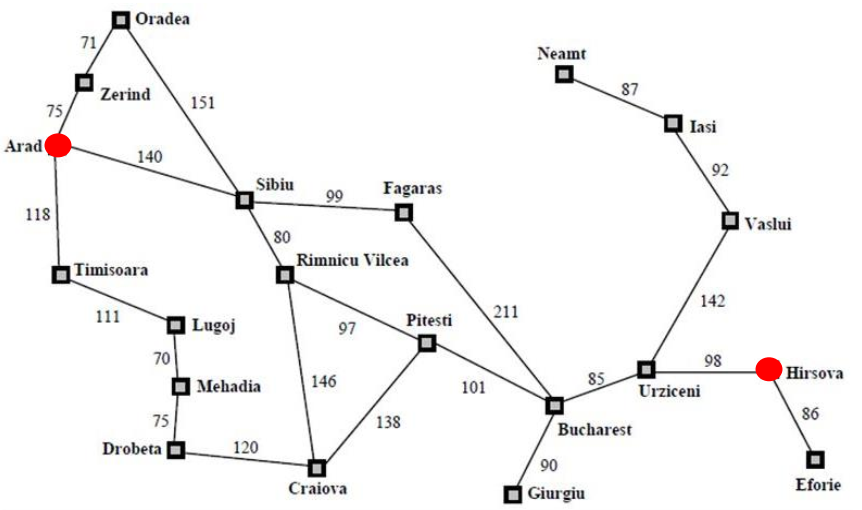
\includegraphics[width=\textwidth,height=\textheight,keepaspectratio]{graph.png}
  \caption{Đồ thị sử dụng đề minh hoạ bài toán tìm đường đi ngắn nhất}
\end{figure}

\clearpage
\section{Giải thuật Heuristic}
\textbf{Heuristic} trong tiếng Hy lạp cổ nghĩa là \textbf{tìm kiếm} hay \textbf{khám phá}. Heuristic là các kỹ thuật dựa trên kinh nghiệm để giải quyết vấn đề, học hỏi hay khám phá nhằm đưa ra một giải pháp gần như là tối ưu. Các phương pháp heuristic được sử dụng nhằm tăng nhanh quá trình tìm kiếm với các phương án, giải pháp hợp lý (gần như là tối ưu) để giảm bớt việc nhận thức vấn đề khi đưa ra quyết định.

Giải thuật heuristic là một sự mở rộng khái niệm thuật toán, thể hiện cách giải bài toán với các đặc tính sau:

\begin{itemize}
  \item Thường tìm được lời giải tốt (nhưng chưa chắc là tốt nhất).
  \item Thường dễ dàng và nhanh chóng đưa ra kết quả hơn so với một số thuật giải tối ưu, do đó có chi phí thấp hơn.
  \item Thường có vẻ khá tự nhiên, gần gũi với suy nghĩ và hành động của con người.
  \item Có nhiều phương pháp để xây dựng một thuật giải Heuristic, trong đó người ta thường đưa vào một số nguyên lý cơ sở sau:
  \begin{itemize}
    \item \textbf{Nguyên lý vét cạn thông minh}: Trong một bài toán tìm kiếm nào đó, khi không gian tìm kiếm lớn, ta thường tìm cách giới hạn lại không gian tìm kiếm hoặc thực hiện một kiểu dò tìm đặc biệt dựa vào đặc thù của bài toán để nhanh chóng tìm ra trạng thái mục tiêu.
    \item \textbf{Nguyên lý tham lam (Greedy)}: Lấy tiêu chuẩn tối ưu (trên phạm vi toàn cục) của bài toán để làm tiêu chuẩn lựa chọn hành động cho phạm vi cục bộ cùa từng bước (hay từng giai đoạn) trong quá trình tìm kiếm lời giải.
    \item \textbf{Nguyên lý thứ tự}: Thực hiện hành động dựa trên một cấu trúc thứ tự hợp lý của không gian khảo sát nhằm nhanh chóng đạt được một lời giải tốt.
    \item \textbf{Hàm Heuristic}: Trong việc xây dựng các thuật giải Heuristic, người ta thường dùng các \textit{Hàm Heuristic}. Đó là các hàm đánh giá thô, giá trị của hàm phụ thuộc vào trạng thái hiện tại của bài toán ở mỗi bước giải. Nhờ giá trị này, ta có thể chọn được cách hành động tương đối hợp lý trong từng bước của thuật giải.
  \end{itemize}
\end{itemize}

\section{Best First Search}
\textbf{Best First Search} là một nhánh thuộc lớp các bài toán tìm kiếm. Theo đó, \textbf{Best First Search} ưu tiên duyệt đồ thị theo trình tự các trạng thái tuân theo một quy luật nào đó.

\textbf{Judea Pearl} (nhà khoa học máy tính sinh năm 1936, người phát triển lý thuyết mạng Bayesian) miêu tả thuật toán \textbf{Best First Search} bằng việc ước lượng khả năng phù hợp của node $n$ bằng một hàm đánh giá $f(n)$ tổng quát dựa trên miêu tả của node $n$, miêu tả của node mục tiêu, tri thức ban đầu có được, và quan trọng nhất, chính là tri thức bổ sung cho bài toán được đặt ra.

Lời giải phù hợp có thể được cài đặt bằng cách sử dụng một hàng đợi ưu tiên (priority queue).

Hai trường hợp đặc biệt của giải thuật \textbf{Best First Search} chính là \textbf{Greedy Best First Search} và \textbf{A* Search}.

\clearpage

\section{Thuật toán Greedy Best First Search (GBFS)}
Thuật toán sử dụng hàm đánh giá $f(n)$ chính là hàm Heuristic $h(n)$. Hàm Heuristic $h(n)$ đánh giá chi phí ước lượng để đi từ node hiện tại $n$ để node đích (mục tiêu). Thuật toán GBFS sẽ ưu tiên xét node "có vẻ" gần với node đích (mục tiêu) nhất.

Mã giả cho thuật toán được thể hiện ở bên dưới:
\begin{vnalgorithm}
  \caption{Thuật toán Greedy Best First Search (GBFS)}
  \begin{algorithmic}[1]
    \INPUT Bài toán.
    \OUTPUT Lời giải hoặc thông báo: Không tồn tại lời giải.
    \STATE {\lstinline|insert(state = initial_state, priority = 0)| \lstinline|into search.queue|;}
    \WHILE{\lstinline|search.queue not empty|}
      \STATE {\lstinline|current_queue.entry = pop item from front of search.queue|}
      \STATE {\lstinline|current_state = current_queue.entry.state|;}
      \STATE {\lstinline|current_heuristic = current_queue.entry.heuristic|;}
      \STATE {\lstinline|starting_counter = counter from current_queue.entry|;}
      \STATE {\lstinline|applicable_actions = array of actions applicable in current_state|;}
      \FOR {\textbf{all} \lstinline|index ?i in applicable_actions >= | \lstinline| starting_counter|}
        \STATE \lstinline|current_action = applicable_actions[?i];|
        \STATE \lstinline|successor_state = current_state.apply(current_action);|
        \IF{\lstinline{successor_state is goal state}}
          \RETURN{\lstinline|solution_path|;}
        \ENDIF
        \STATE{\lstinline|successor_heuristic = heuristic value of successor_state|;}
        \IF{\lstinline{successor_heuristic < current_heuristic}}
          \STATE {\lstinline|insert(current_state, current_heuristic, ?i + 1)| \lstinline|to search.queue|;}
          \STATE {\lstinline|insert(successor_state, successor_heuristic, 0)| \lstinline|to search.queue|;}
          \STATE \textbf{break for;}
        \ELSE
          \STATE {\lstinline|insert(successor_state, successor_heuristic, 0)| \lstinline|to search.queue|;}
        \ENDIF
      \ENDFOR
    \ENDWHILE
    
  \end{algorithmic}
\end{vnalgorithm}

Ví dụ, đối với đồ thị ở hình 1, giả sử ta có hàm Heuristic $h(n)$ được xác định như ở bảng sau:

\begin{center}
  \begin{tabular}{ |c|c|c|c| }
    \hline
    $h(\text{Arad}) = 366$ & $h(\text{Bucharest}) = 20$ & $h(\text{Craiova}) = 160$ & $h(\text{Drobeta}) = 242$ \\
    \hline
    $h(\text{Eforie}) = 161$ & $h(\text{Fagaras}) = 176$ & $h(\text{Giurgiu}) = 77$ & $h(\text{Hirsova}) = 0$ \\
    \hline
    $h(\text{Iasi}) = 226$ & $h(\text{Lugoj}) = 244$ & $h(\text{Mehadia}) = 241$ & $h(\text{Neamt}) = 234$ \\
    \hline
    $h(\text{Oradea}) = 380$ & $h(\text{Pitesti}) = 100$ & $h(\text{Rimnicu Vilcea}) = 193$ & $h(\text{Sibiu}) = 253$ \\
    \hline
    $h(\text{Timisoara}) = 329$ & $h(\text{Urziceni}) = 10$ & $h(\text{Vaslui}) = 199$ & $h(\text{Zerind}) = 374$ \\
    \hline
  \end{tabular}
\end{center}

Áp dụng thuật toán GBFS, ta có lời giải cho bài toán tìm đường đi ngắn nhất từ Arad (1) đến Hirsova (8) được thể hiện như bảng sau:

\begin{center}
  \begin{tabular}{ |c|c|c|c| }
    \hline
    \textbf{Lần lặp} & \textbf{Đỉnh} & \textbf{Hàng đợi ưu tiên (theo thứ tự hàm $h(n)$)} & \textbf{Tổng chi phí $f(n)$} \\
    \hline
    0 & $\emptyset$ & (1, 366)* & $0$ \\
    \hline
    1 & 1 & (16, 253)*, (17, 329), (1, 366), (20, 374) & $0 + 140 = 140$\\
    \hline
    2 & 16 & (6, 176)*, (15, 193), (1, 366), (15, 380) & $140 + 99 = 239 $\\
    \hline
    3 & 6 & (2, 20)*, (16, 253) & $239 + 211 = 450$\\
    \hline
    4 & 2 & (14, 10)*, (7, 77), (6, 176) & $450 + 85 = 535$\\
    \hline
    5 & 14 & (8, 0)*, (2, 20), (19, 199) & $535 + 98 = 633$\\
    \hline
  \end{tabular}
\end{center}
Vậy đường đi ngắn nhất từ Arad đến Hirsova thông qua thuật toán GBFS là:
\begin{center}
  Arad $\xrightarrow{140}$ Sibiu $\xrightarrow{99}$ Fagaras $\xrightarrow{211}$ Bucharest $\xrightarrow{85}$ Urziceni $\xrightarrow{98}$  Hirsova
\end{center}

\section{Thuật toán A-star (A*)}
A* là một giải thuật tìm kiếm trong đồ thị, tìm đường đi từ một đỉnh hiện tại đén đỉnh đích có sử dụng hàm để ước lượng khoảng cách. Hàm ước lượng này có dạng $f(n) = g(n) + h(n)$, trong đó:
\begin{itemize}
  \item $g(n)$ là chi phí đi từ node gốc đến node đó.
  \item $h(n)$ là chi phí ước lượng từ node đó đến node đích.
\end{itemize}
Mã giả cho thuật toán A* được mô tả như ở trang 8. 

Áp dụng thuật toán A* kết hợp với hàm Heuristic $h(n)$ đã cho ở mục 4.1, ta có lời giải cho bài toán tìm đường đi ngắn nhất từ Arad (1) đến Hirsova (8) được thể hiện như sau: (Mỗi node trong tập OPEN và CLOSE được thể hiện bởi 5 giá trị: số thứ tự của thành phố, giá trị hàm $g(n)$, giá trị hàm $h(n)$ giá trị hàm $h(n)$ và số thứ tự của node cha tương ứng).

Sau khi kết thúc thuật toán, ta thu được đường đi ngắn nhất từ Arad đến Hirsova theo thuật toán A* là
\begin{center}
  Arad $\xrightarrow{140}$ Sibiu $\xrightarrow{80}$ Rimincu Vilcea $\xrightarrow{97}$ Pitesti $\xrightarrow{101}$ Bucharest $\xrightarrow{85}$ Urziceni $\xrightarrow{98}$ Hirsova
\end{center}

\clearpage
\begin{center}
  \begin{tabular}{ |c|c|c| }
    \hline
    Lần lặp  & OPEN & CLOSE \\
    \hline
    0 & (1, 0, 0, 0, $\emptyset$)* & $\emptyset$ \\
    \hline
      1 & (16, 140, 253, 393, 1)* & (1, 0, 0, 0, $\emptyset$)\\
      & (17, 118, 329, 447, 1) & \\
      & (20, 75, 374, 449, 1) & \\
    \hline
      2 & (17, 118, 329, 447, 1)& (1, 0, 0, 0, $\emptyset$) \\ 
      & (20, 75, 374, 449, 1) & (16, 140, 253, 393, 1)\\
      & (15, 220, 193, 413, 16)*  & \\
      & (6, 239, 176, 415, 16)& \\
      & (1, 280, 366, 646, 16) & \\
      & (13, 291, 380, 671, 16) & \\
    \hline
      3 & (17, 118, 329, 447, 1) & (1, 0, 0, 0, $\emptyset$) \\
      & (20, 75, 374, 449, 1)& (16, 140, 253, 393, 1)\\
      & (6, 239, 176, 415, 16)*& (15, 220, 193, 413, 16)\\
      & (1, 280, 366, 646, 16) & \\
      & (13, 291, 380, 671, 16) & \\
      & (14, 317, 100, 417, 15) & \\
      & (3, 366, 160, 526, 15) & \\
      & (16, 300, 253, 553, 15) &\\
    \hline
      4 & (17, 118, 329, 447, 1) & (1, 0, 0, 0, $\emptyset$)\\
      & (20, 75, 374, 449, 1) & (16, 140, 253, 393, 1)\\
      & (1, 280, 366, 646, 16) & (15, 220, 193, 413, 16)\\
      & (13, 291, 380, 671, 16) & \\
      & (14, 317, 100, 417, 15)* & \\
      & (3, 366, 160, 526, 15) & \\
      & (16, 300, 253, 553, 15) &\\
      & (2, 450, 0, 450, 6) & \\
    \hline
      5 & (17, 118, 329, 447, 1) & (1, 0, 0, 0, $\emptyset$)\\
      & (20, 75, 374, 449, 1) & (16, 140, 253, 393, 1)\\
      & (1, 280, 366, 646, 16) & (15, 220, 193, 413, 16)\\
      & (13, 291, 380, 671, 16) & (14, 317, 100, 417, 15)\\
      & (3, 366, 160, 526, 15) & \\
      & (16, 300, 253, 553, 15) & \\
      & (2, 418, 0, 418, 6)* & \\
      & (15, 414, 193, 604, 14) & \\
    \hline
      6 & (17, 118, 329, 447, 1)* & (1, 0, 0, 0, $\emptyset$)\\
      & (20, 75, 374, 449, 1) & (16, 140, 253, 393, 1)\\
      & (1, 280, 366, 646, 16) & (15, 220, 193, 413, 16)\\
      & (13, 291, 380, 671, 16) & (14, 317, 100, 417, 15)\\
      & (3, 366, 160, 526, 15) & (2, 418, 0, 418, 6)\\
      & (16, 300, 253, 553, 15) & \\
      & (15, 414, 193, 604, 14) & \\
      & (6, 629, 176, 805, 2)& \\
      & (7, 508, 77, 585, 2) & \\
      & (18, 503, 10, 513, 2) & \\
    \hline
  \end{tabular}
\end{center}


\begin{center}
  \begin{tabular}{ |c|c|c| }
    \hline
    Lần lặp & OPEN & CLOSE \\
    \hline
      7 & (20, 75, 374, 449, 1)* & (1, 0, 0, 0, $\emptyset$)\\
      & (1, 280, 366, 565, 17) & (16, 140, 253, 393, 1)\\
      & (13, 291, 380, 671, 16) & (15, 220, 193, 413, 16)\\
      & (3, 366, 160, 526, 15) & (14, 317, 100, 417, 15)\\
      & (16, 300, 253, 553, 15) & (2, 418, 0, 418, 6)\\
      & (15, 414, 193, 604, 14) & (17, 118, 329, 447, 1)\\
      & (6, 629, 176, 805, 2) & \\
      & (7, 508, 77, 585, 2) & \\
      & (18, 503, 10, 513, 2) & \\
      & (10, 299, 244, 543, 17) & \\
    \hline
      8 & (1, 280, 366, 524, 20) & (1, 0, 0, 0, $\emptyset$)\\
      & (13, 291, 380, 671, 16) & (16, 140, 253, 393, 1)\\
      & (3, 366, 160, 526, 15) & (15, 220, 193, 413, 16)\\
      & (16, 300, 253, 553, 15) & (14, 317, 100, 417, 15)\\
      & (15, 414, 193, 604, 14) & (2, 418, 0, 418, 6)\\
      & (6, 629, 176, 805, 2) & \\
      & (7, 508, 77, 585, 2) & \\
      & (18, 503, 10, 513, 2)* & \\
      & (10, 299, 244, 543, 17) & \\
      & (13, 146, 380, 526, 20)& \\
    \hline
      9 & (1, 280, 366, 524, 20) & (1, 0, 0, 0, $\emptyset$)\\
      & (13, 291, 380, 671, 16) & (16, 140, 253, 393, 1)\\
      & (3, 366, 160, 526, 15) & (15, 220, 193, 413, 16)\\
      & (16, 300, 253, 553, 15) & (14, 317, 100, 417, 15)\\
      & (15, 414, 193, 604, 14) & (2, 418, 0, 418, 6)\\
      & (6, 629, 176, 805, 2) & (18, 503, 10, 513, 2)\\
      & (7, 508, 77, 585, 2) & \\
      & (10, 299, 244, 543, 17) & \\
      & (13, 146, 380, 526, 20) & \\
      & (2, 588, 20, 608, 18) & \\
      & (8, 601, 0, 601, 18) (dừng) & \\
    \hline
  \end{tabular}
\end{center}


\begin{vnalgorithm}
  \caption{Thuật toán A*}
  \begin{algorithmic}[1]
    \INPUT Bài toán.
    \OUTPUT Lời giải hoặc thông báo: Không tồn tại lời giải.
    \STATE {$\text{OPEN} = T_0$}
    \STATE {$g(T_0) = 0, h(T_0) = 0, f(T_0) = 0$}
    \STATE {$\text{CLOSE} = \emptyset$}
    \LOOP
      \IF{$\text{OPEN}$ rỗng}
        \STATE {Bài toán vô nghiệm.}
        \STATE \textbf{exit}
      \ELSE
        \STATE {Lấy $T_{\text{max}}$ ra khỏi OPEN}
        \STATE {Đưa $T_{\text{max}}$ vào CLOSE}
        \IF{$T_{\text{max}}$ là trạng thái đích}
          \STATE{Lời giải là $T_{\text{max}}$}
          \STATE \textbf{exit}
        \ELSE
          \STATE {Tạo danh sách tất cả các trạng thái kế tiếp $T_K$ của $T_{\text{max}}$}
          \FOR {\textbf{each} $T_K$}
            \STATE {$g(T_K) = g(T_{\text{max}}) + \text{cost}(T_{\text{max}}, T_K)$}
            \IF{tồn tại $T_{K'}$ trong OPEN trùng với $T_K$}
              \IF{$g(T_K) < g(T_{K'})$}
                \STATE {$g(T_{K'}) = g(T_K)$}
                \STATE {Tính lại $f(T_{K'})$}
                \STATE {FATHER($T_{K'}$) = $T_{\text{max}}$}
              \ENDIF
            \ENDIF
            \IF{tồn tại $T_{K'}$ trong CLOSE trùng với $T_K$}
              \IF{$g(T_K) < g(T_{K'})$}
                \STATE {$g(T_{K'}) = g(T_K)$}
                \STATE {Tính lại $f(T_{K'})$}
                \STATE {FATHER($T_{K'}$) = $T_{\text{max}}$}
              \ENDIF
            \ENDIF
            \STATE{\textit{Lan truyền} sự thay đổi của $f$ và $g$ cho tất cả các trạng thái kế tiếp của $T_i$ (ở tất cả các cấp) đã được lưu trữ trong CLOSE và OPEN.}
            \IF{$T_K$ chưa xuất hiện trong cả OPEN và CLOSE}
              \STATE{Thêm $T_K$ vào OPEN}
              \STATE{$f(T_K) = g(T_K) + h(T_K)$}
            \ENDIF
          \ENDFOR
        \ENDIF  
      \ENDIF
    \ENDLOOP
  \end{algorithmic}
\end{vnalgorithm}

\clearpage

\section{Cài đặt bằng \lstinline|Python| }
Trong phần này chúng ta sẽ đi vào chi tiết cách cài đặt chương trình Python để giải quyết bài toán được đặt ở phần 1. File chương trình có tên là \lstinline|program.py|. Chương trình được viết bằng ngôn ngữ \lstinline|Python| và sử dụng thư viện \lstinline|matplotlib| để vẽ giao diện. Chương trình được chia thành 2 phần chính: các hàm và hàm \lstinline|main|.

\subsection{Cấu trúc file đầu vào}
Có ba file đầu vào cho chương trình. File đầu tiên là file \lstinline|cities.txt|. Mỗi dòng trong file gồm 3 thành phần phân cách nhau bởi khoảng trắng. Thành phần đầu tiên là tên thành phố, 2 thành phần còn lại chính là toạ độ của thành phố đó (hình 2a).

File thứ hai là \lstinline|citiesGraph.txt| gồm 3 thành phần phân cách nhau bởi khoảng trắng. Thành phần đầu tiên là tên thành phố, thành phần thứ hai là tên thành phố kề với thành phố đầu tiên, thành phần thứ ba là khoảng cách giữa hai thành phố đó (hình 2b).

File cuối cùng là \lstinline|heuristic.txt| gồm 2 thành phần phân cách nhau bởi khoảng trắng. Thành phần đầu tiên là tên thành phố, thành phần thứ hai là hàm Heuristic khoảng cách từ thành phố đó đến thành phố đích (hình 2c).

\begin{figure}[h]
  \centering\
  \begin{subfigure}[b]{0.3\textwidth}
    \centering
    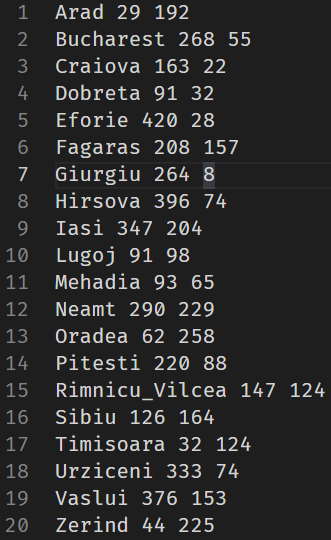
\includegraphics[width=\textwidth,height=\textheight,keepaspectratio]{cities.png}
    \caption{\lstinline|cities.txt| }
  \end{subfigure}
  \hfill
  \begin{subfigure}[b]{0.3\textwidth}
    \centering
    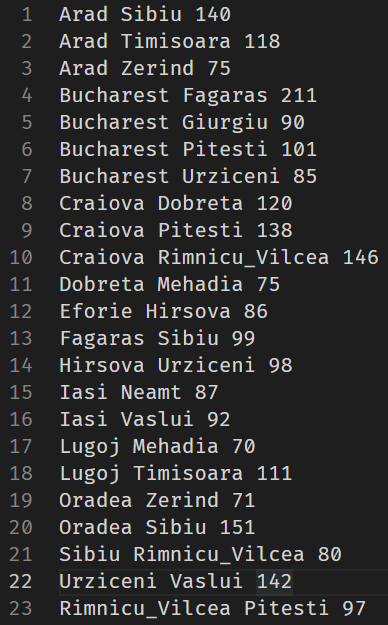
\includegraphics[width=\textwidth,height=\textheight,keepaspectratio]{citiesGraph.png}
    \caption{\lstinline|citiesGraph.txt| }
  \end{subfigure}
  \hfill
  \begin{subfigure}[b]{0.3\textwidth}
    \centering
    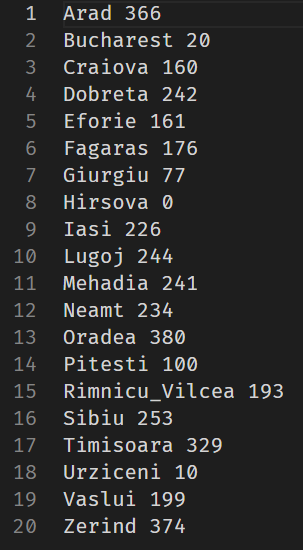
\includegraphics[width=\textwidth,height=\textheight,keepaspectratio]{heuristic.png}
    \caption{\lstinline|heuristic.txt| }
  \end{subfigure}
  \caption{Các file đầu vào}
\end{figure}


\subsection{Các hàm}
\begin{itemize}
  \item \lstinline|getHeuristics()|: đọc dữ liệu từ file \lstinline|heuristics.txt| và lưu vào \lstinline|dictionary| tên là \lstinline|heuristics| với \lstinline|key| là tên thành phố và \lstinline|value| là hàm Heuristic của thành phố đó.
  \item \lstinline|getCity()|: đọc dữ liệu từ file \lstinline|cities.txt| và lưu vào 2 \lstinline|dictionary| tên là \lstinline|city| và \lstinline|cityCode|:
  \begin{itemize}
    \item Đối với \lstinline|city|, \lstinline|key| là tên thành phố và \lstinline|value| là một \lstinline|list| gồm toạ độ của thành phố đó.
    \item Đối với \lstinline|cityCode|, \lstinline|key| là số thứ tự cùa hàng chứa tên thành phố đó và \lstinline|value| là tên thành phố đó.
  \end{itemize}
  \item \lstinline|createGraph()|: đọc dữ liệu từ file \lstinline|citiesGraph.txt| và lưu vào \lstinline|dictionary| tên là \lstinline|graph| với \lstinline|key| là tên thành phố và \lstinline|value| là một \lstinline|list| gồm tên thành phố kề với nó và khoảng cách giữa hai thành phố đó.
  \item \lstinline|drawMap(city, gbfs, astar, graph)|: mô phỏng đồ thị của bài toán cũng như lời giải cho hai thuật toán GBFS và A*.
  \item \lstinline|GBFS(startNode, heuristics, graph, goalNode)|: thực thi thuật toán Greedy Best First Search với node bắt đầu \lstinline|startNode|, giá trị hàm Heuristics \lstinline|heuristics|, đồ thị \lstinline|graph| và node đích \lstinline|endNode|.
  \item \lstinline|Astar(startNode, heuristics, graph, goalNode)|: thực thi thuật toán A-star với node bắt đầu \lstinline|startNode|, giá trị hàm Heuristics \lstinline|heuristics|, đồ thị \lstinline|graph| và node đích \lstinline|endNode|.
\end{itemize}

\subsection{Hàm \lstinline|main|}
Nhiệm vụ của hàm main là mô phỏng lại bài toán tìm đường đi ngắn nhất đã được miêu trả ở mục 1. Chương trình sẽ dừng lại khi người dùng nhập giá trị của đỉnh bắt đầu hoặc đỉnh kết thúc là 0:
\begin{lstlisting}[language=Python]
if __name__ ==  "__main__":
  heuristic = getHeuristics()
  graph = createGraph()
  city, citiesCode = getCity()

  print(heuristic)

  for i, j in citiesCode.items():
      print(i, j)
      
  while True:
      inputCode1 = int(input("Nhap dinh bat dau: "))
      inputCode2 = int(input("Nhap dinh ket thuc: "))

      if inputCode1 == 0 or inputCode2 == 0:
          break

      startCity = citiesCode[inputCode1]
      endCity = citiesCode[inputCode2]

      gbfs = GBFS(startCity, heuristic, graph, endCity)
      astar = Astar(startCity, heuristic, graph, endCity)
      print("GBFS => ", gbfs)
      print("ASTAR =>", astar)

      drawMap(city, gbfs, astar, graph)
\end{lstlisting}


\subsection{Kết quả}
Sau khi chạy chương trình trên, ta thu được kết quả đường đi ngắn nhất từ Arad đến Hirsova như hình 3 và được mô phỏng như hình 4:
\begin{figure}[ht]
  \centering
  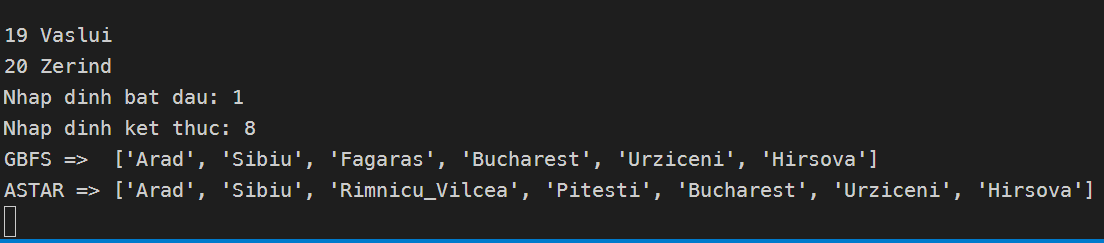
\includegraphics[width=\textwidth,height=\textheight,keepaspectratio]{terminal_result.png}
  \caption{Kết quả đường đi ngắn nhất từ Arad đến Hirsova bằng Terminal}
\end{figure}
\begin{figure}[ht]
  \centering
  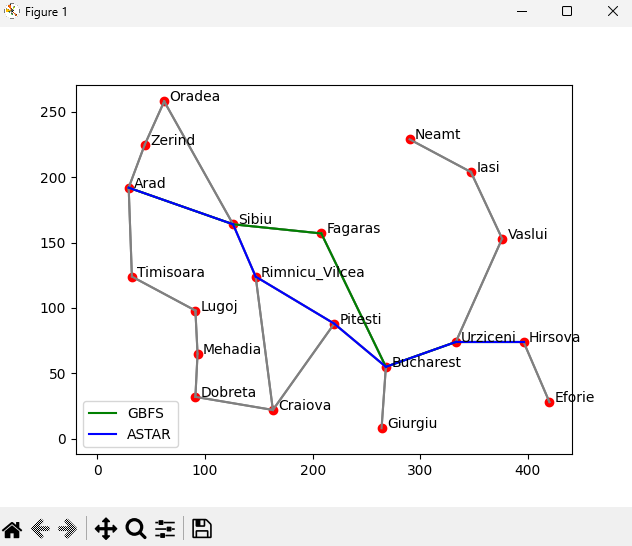
\includegraphics[width=.75\textwidth,height=.75\textheight,keepaspectratio]{figure_result.png}
  \caption{Mô phỏng đường đi ngắn nhất từ Arad đến Hirsova bằng Matplotlib}
\end{figure}
\clearpage


\section{Nhận xét}
\begin{itemize}
  \item Hai thuật toán sử dụng hai hàm đánh giá khác nhau: đối với GBFS là $f(n) = h(n)$ còn đối với A* là $f(n) = g(n) + h(n)$.
  \item Thuật toán GBFS là thuật toán \textbf{không hoàn thiện} vì thuật toán này không đảm bảo ta sẽ tìm được dường đi từ node bắt đầu đến node đích. Trái lại, thuật toán A* là thuật toán \textbf{hoàn thiện} vì thuật toán này luôn đảm bảo đường đi từ node bắt đầu đến node kết thúc là có thể tìm được.
  \item Thuật toán GBFS tốn ít bộ nhớ hơn, vì các node sau khi được duyệt sẽ luôn được đẩy ra sau mỗi bước lặp. Trong khi đó, thuật toán A* cần phải lưu lại vết của các node đã được duyệt để có thể truy vết lại đường đi ngắn nhất.
  \item Thuật toán GBFS là thuật toán \textbf{không tối ưu}, nghĩa là đường đi tìm được có thể không phải là đường đi ngắn nhất. Ngược lại, thuật toán A* là thuật toán \textbf{tối ưu} vì ta luôn tìm được đường đi ngắn nhất từ node bắt đầu đến node kết thúc.
  \item Cả hai thuật toán đều có độ phức tạp thời gian là $\mathcal{O}(b^m)$ với $b$ là số lượng node con (tối đa) của mỗi node và $m$ là chiều sâu tối đa của cây tìm kiếm.
  \item Trên thực tế, người ta thường dùng một thuật toán khác để tìm đường đi ngắn nhất, ví dụ như thuật toán Iterative Deepening A* - IDA* với độ phức tạp $\mathcal{O}(d)$ với $d$ là độ sâu của cây.
\end{itemize}


\section{Tham khảo}
\begin{enumerate}
  \item Stuart J. Russell, Peter Norvig (2010), Aritificial Intelligence: A Modern Approach, 3rd Edition, Prentice Hall, ISBN-13: 978-0-13-604259-4, ISBN-10: 0-13-604259-7 (\url{https://zoo.cs.yale.edu/classes/cs470/materials/aima2010.pdf})
  \item Greedy Best-First Search - GBFS (2019), \url{https://www.geeksforgeeks.org/greedy-best-first-search-gbfs/}
  \item A* Search Algorithm (2019), \url{https://www.geeksforgeeks.org/a-search-algorithm/}
  \item Iterative Deepening A* - IDA* (\url{https://en.wikipedia.org/wiki/Iterative_deepening_A*})
\end{enumerate}
\pagebreak
\end{document}